%-----------------------------------------------------------------------------%
\chapter{\babLima}
%-----------------------------------------------------------------------------%

Bab ini menjelaskan hasil pengujian yang dilakukan terhadap perangkat yang dibuat untuk menguji apakah hasil implementasi berjalan sesuai seperti yang diharapkan atau tidak. Penjelasan meliputi perangkat yang digunakan dan hasil pengujian.

\section{Perangkat yang Digunakan}

Perangkat yang digunakan dalam pengujian ini adalah dua buah lampu yang akan dikontrol. Masing-masing lampu ini adalah sebuah lampu berbasis ZigBee dengan merek Philips Hue. Philips Hue adalah sebuah lampu ZigBee yang mengimplementasikan profil ZigBee \textit{Light Link}. Philips Hue merupakan sebuah \textit{Color Dimmable Light}, sehingga dapat diubah warnanya dan tingkat kecerahannya. Gambar \ref{fig:philips-hue} menunujukkan foto kedua lampu yang digunakan.

\begin{figure}
	\centering
	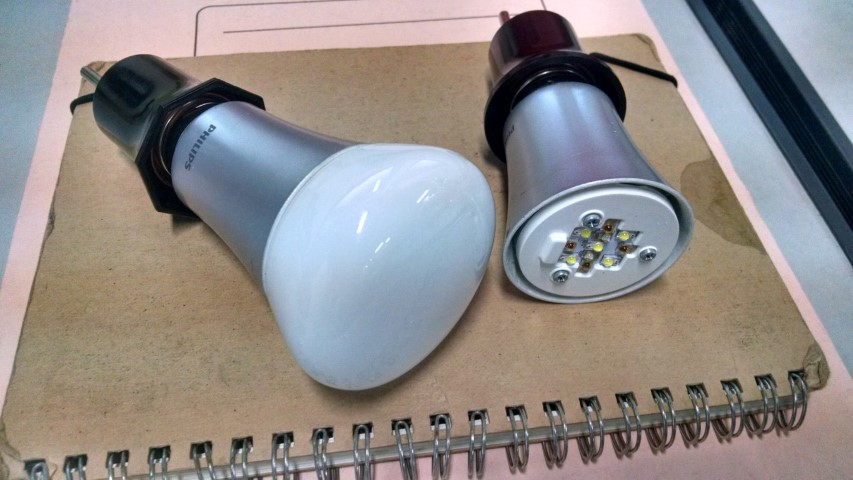
\includegraphics[width=.9\textwidth]{pics/philips-hue.jpg}
	\caption{Lampu Philips Hue yang digunakan untuk pengujian}
	\label{fig:philips-hue}
\end{figure}

\subsection{Hasil Pengujian}
\begin{enumerate}
	\item Kasus Uji 1: Menjadi \textit{access point}.
	\begin{table}
		\centering
		\caption{Hasil pengujian kasus uji 1}
		\label{tab:kasusUji1}
		\begin{tabular}{| l | p{11cm} |}
			\hline
			\textbf{Perintah} & Perangkat \textit{gateway} dinyalakan \\
			\hline
			\textbf{Prekondisi} & -\\
			\hline
			\textbf{Hasil} & Perangkat \textit{gateway} menyala dengan \textit{access point} bernama "ZigBee\_Gateway" muncul
			
			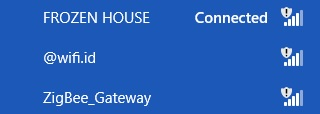
\includegraphics[width=.65\textwidth]{pics/uji1.jpg}\\
			\hline
			\textbf{Ekspektasi} & \textit{Access point} bernama "ZigBee\_Gateway" muncul \\
			\hline
		\end{tabular}
	\end{table}
	\item Kasus Uji 2: Menghubungkan perangkat \textit{gateway} ke \textit{access point} lain.
	\begin{table}
		\centering
		\caption{Hasil pengujian kasus uji 2}
		\label{tab:kasusUji2}
		\begin{tabular}{| l | p{11cm} |}
			\hline
			\textbf{Perintah} & Membuka halaman \code{192.168.42.1/ta/wifi.php}, dan memilih salah satu \textit{access point} lain \\
			\hline
			\textbf{Prekondisi} & Perangkat yang digunakan untuk mengakses sudah terhubung ke perangkat \textit{gateway}\\
			\hline
			\textbf{Hasil} & Perangkat \textit{gateway} terhubung ke \textit{access point} yang dipilih dan mendapatkan alamat IP \code{192.168.1.135}.
			
			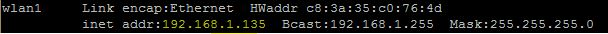
\includegraphics[width=.65\textwidth]{pics/uji1x.jpg}\\
			\hline
			\textbf{Ekspektasi} & Perangkat \textit{gateway} terhubung ke \textit{access point} yang dipilih dan mendapatkan sebuah alamat IP \\
			\hline
		\end{tabular}
	\end{table}
	\item Kasus Uji 3: Menyalakan lampu melalui halaman web pada perangkat \textit{gateway}
	\begin{table}
		\centering
		\caption{Hasil pengujian kasus uji 3}
		\label{tab:kasusUji3}
		\begin{tabular}{| l | p{11cm} |}
			\hline
			\textbf{Perintah} & Tombol 'Nyalakan' ditekan \\
			\hline
			\textbf{Prekondisi} & Perangkat \textit{gateway} sudah berjalan, lampu sudah terhubung dengan perangkat \textit{gateway} dan dalam keadaan mati\\
			\hline
			\textbf{Hasil} & Lampu menyala 
			
			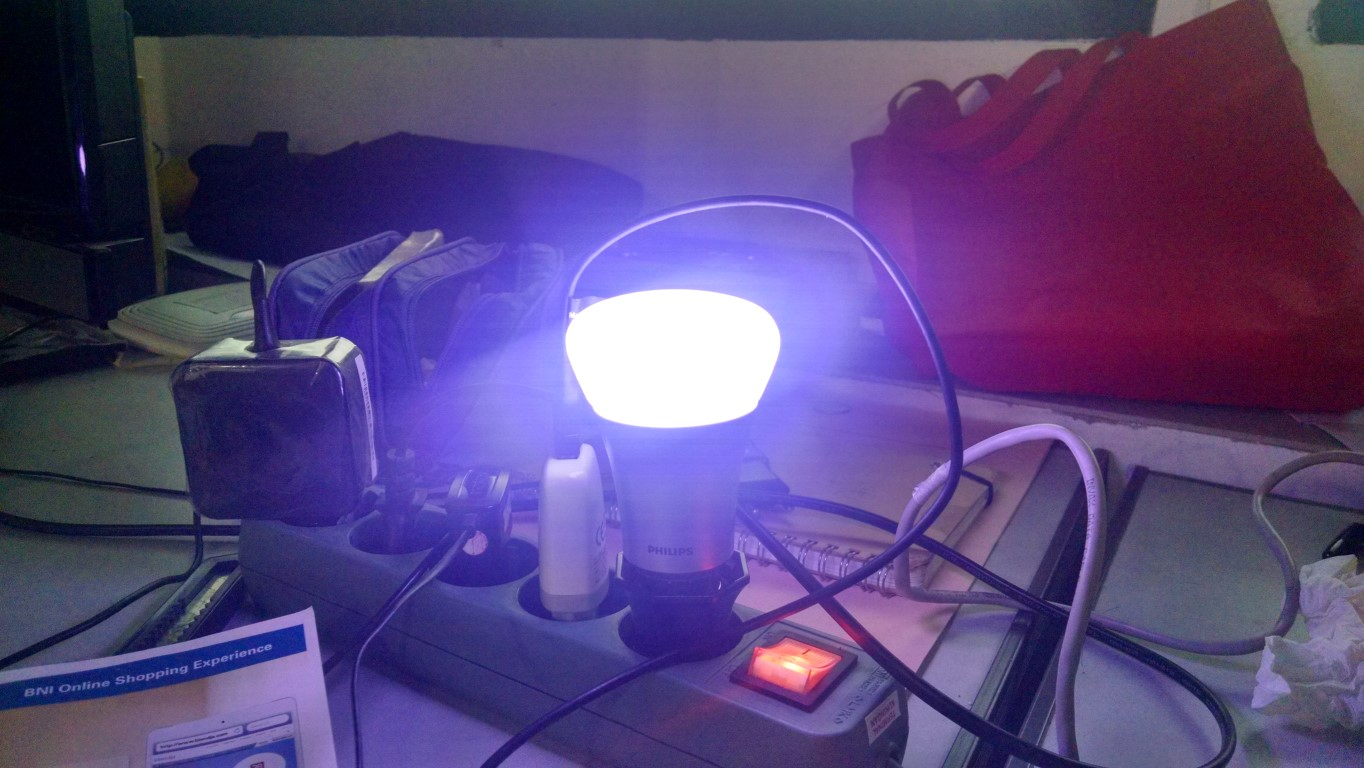
\includegraphics[width=.65\textwidth]{pics/uji2.jpg}\\
			\hline
			\textbf{Ekspektasi} & Lampu menyala \\
			\hline
		\end{tabular}
	\end{table}
	\item Kasus Uji 4: Mematikan lampu melalui halaman web pada perangkat \textit{gateway}
	\begin{table}
		\centering
		\caption{Hasil pengujian kasus uji 4}
		\label{tab:kasusUji4}
		\begin{tabular}{| l | p{11cm} |}
			\hline
			\textbf{Perintah} & Tombol 'Matikan' ditekan \\
			\hline
			\textbf{Prekondisi} & Perangkat \textit{gateway} sudah berjalan, lampu sudah terhubung dengan perangkat  \textit{gateway} dan dalam keadaan menyala\\
			\hline
			\textbf{Hasil} & Lampu mati 
			
			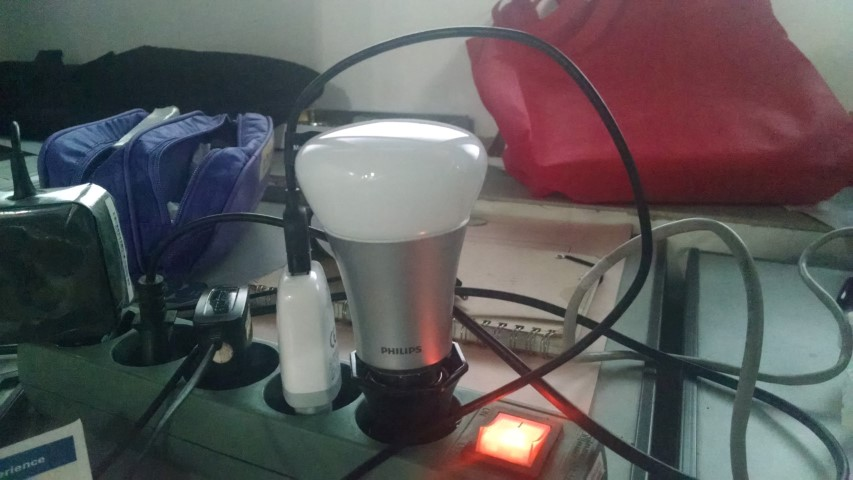
\includegraphics[width=.65\textwidth]{pics/uji3.jpg}\\
			\hline
			\textbf{Ekspektasi} & Lampu mati \\
			\hline
		\end{tabular}
	\end{table}
	\item Kasus Uji 5: Mengubah tingkat kecerahan lampu melalui halaman web pada perangkat \textit{gateway}
	\begin{table}
		\centering
		\caption{Hasil pengujian kasus uji 5}
		\label{tab:kasusUji5}
		\begin{tabular}{| l | p{11cm} |}
			\hline
			\textbf{Perintah} & \textit{Slider} tingkat kecerahan digeser ke nilai yang lebih tinggi \\
			\hline
			\textbf{Prekondisi} & Perangkat \textit{gateway} sudah berjalan, lampu sudah terhubung dengan perangkat  \textit{gateway} dan dalam keadaan menyala\\
			\hline
			\textbf{Hasil} & Lampu menjadi lebih terang 
			
			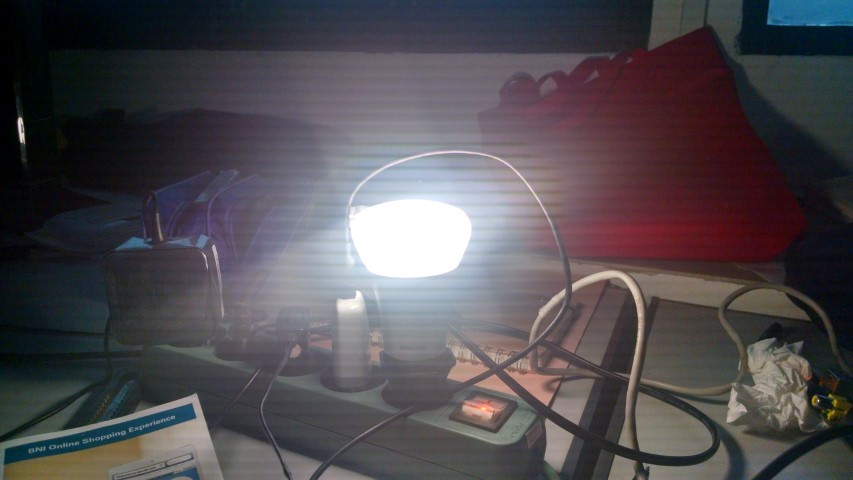
\includegraphics[width=.65\textwidth]{pics/uji4.jpg}\\
			\hline
			\textbf{Ekspektasi} & Lampu menjadi lebih terang \\
			\hline
		\end{tabular}
	\end{table}
	\item Kasus Uji 6: Mengubah warna lampu melalui halaman web pada perangkat \textit{gateway}
	\begin{table}
		\centering
		\caption{Hasil pengujian kasus uji 6}
		\label{tab:kasusUji6}
		\begin{tabular}{| l | p{11cm} |}
			\hline
			\textbf{Perintah} & Mengubah warna pada \textit{color picker} menjadi berwarna merah \\
			\hline
			\textbf{Prekondisi} & Perangkat \textit{gateway} sudah berjalan, lampu sudah terhubung dengan perangkat  \textit{gateway} dan dalam keadaan menyala\\
			\hline
			\textbf{Hasil} & Lampu menjadi berwarna merah 
			
			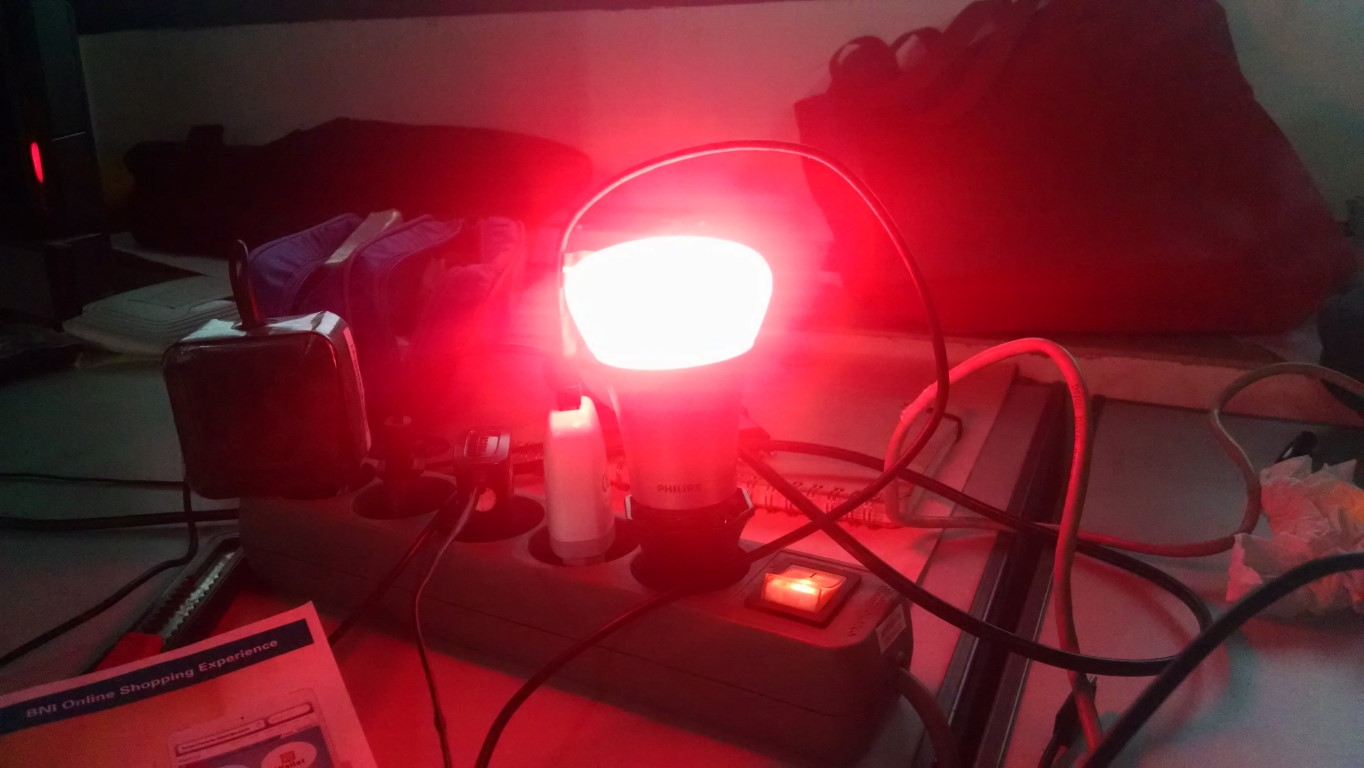
\includegraphics[width=.65\textwidth]{pics/uji5.jpg}\\
			\hline
			\textbf{Ekspektasi} & Lampu menjadi berwarna merah \\
			\hline
		\end{tabular}
	\end{table}
	\item Kasus Uji 7: Mengubah tingkat kejenuhan lampu melalui halaman web pada perangkat \textit{gateway}
	\begin{table}
		\centering
		\caption{Hasil pengujian kasus uji 7}
		\label{tab:kasusUji7}
		\begin{tabular}{| l | p{11cm} |}
			\hline
			\textbf{Perintah} & Menurunkan tingkat kejenuhan warna menggunakan \textit{color picker} \\
			\hline
			\textbf{Prekondisi} & Perangkat \textit{gateway} sudah berjalan, lampu sudah terhubung dengan perangkat  \textit{gateway} dan dalam keadaan menyala\\
			\hline
			\textbf{Hasil} & Lampu menjadi berwarna lebih muda 
			
			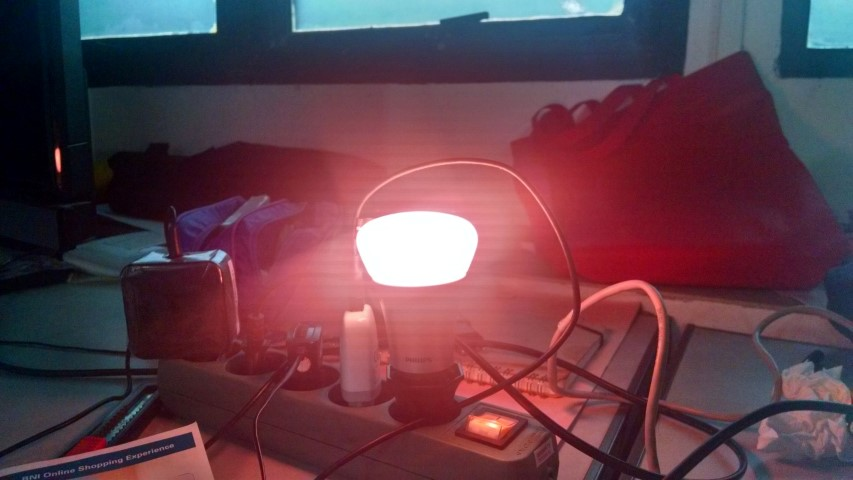
\includegraphics[width=.65\textwidth]{pics/uji6.jpg}\\
			\hline
			\textbf{Ekspektasi} & Lampu menjadi berwarna lebih muda \\
			\hline
		\end{tabular}
	\end{table}
	\item Kasus Uji 8: Membuat sebuah \textit{group} melalui halaman web pada perangkat \textit{gateway}
	\begin{table}
		\centering
		\caption{Hasil pengujian kasus uji 8}
		\label{tab:kasusUji8}
		\begin{tabular}{| l | p{11cm} |}
			\hline
			\textbf{Perintah} & Menekan tombol 'Buat Group', mengisi nama, kemudian memilih 'Light 1' dan 'Light 2', dan menekan tombol 'submit' \\
			\hline
			\textbf{Prekondisi} & Perangkat \textit{gateway} sudah berjalan, lampu sudah terhubung dengan perangkat \textit{gateway}\\
			\hline
			\textbf{Hasil} & Group terdaftar dengan anggota 'Light 1' dan 'Light 2'\\
			\hline
			\textbf{Ekspektasi} & Group terdaftar dengan anggota 'Light 1' dan 'Light 2' \\
			\hline
		\end{tabular}
	\end{table}
	\item Kasus Uji 9: Menyalakan lampu dalam suatu \textit{group} melalui halaman web pada perangkat \textit{gateway}
	\begin{table}
		\centering
		\caption{Hasil pengujian kasus uji 9}
		\label{tab:kasusUji9}
		\begin{tabular}{| l | p{11cm} |}
			\hline
			\textbf{Perintah} & Tombol 'Nyalakan' pada bagian \textit{groups} ditekan \\
			\hline
			\textbf{Prekondisi} & Perangkat \textit{gateway} sudah berjalan, lampu sudah terhubung dengan perangkat \textit{gateway}, \textit{group} sudah dibuat, dan lampu dalam keadaan mati \\
			\hline
			\textbf{Hasil} & Kedua lampu menyala 
			
			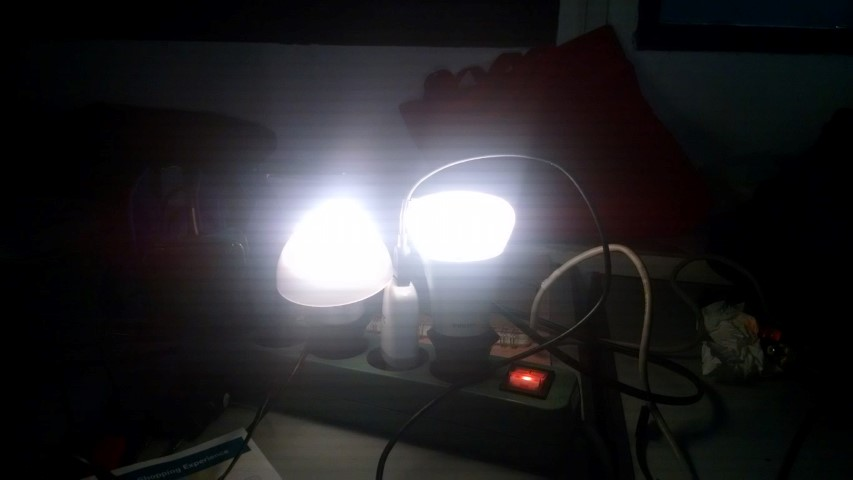
\includegraphics[width=.65\textwidth]{pics/uji8.jpg}\\
			\hline
			\textbf{Ekspektasi} & Kedua lampu menyala \\
			\hline
		\end{tabular}
	\end{table}
	\item Kasus Uji 10: Mematikan lampu dalam suatu \textit{group} melalui halaman web pada perangkat \textit{gateway}
	\begin{table}
		\centering
		\caption{Hasil pengujian kasus uji 10}
		\label{tab:kasusUji10}
		\begin{tabular}{| l | p{11cm} |}
			\hline
			\textbf{Perintah} & Tombol 'Matikan' pada bagian \textit{groups} ditekan \\
			\hline
			\textbf{Prekondisi} & Perangkat \textit{gateway} sudah berjalan, lampu sudah terhubung dengan perangkat \textit{gateway}, \textit{group} sudah dibuat, dan lampu dalam keadaan menyala \\
			\hline
			\textbf{Hasil} & Kedua lampu mati 
			
			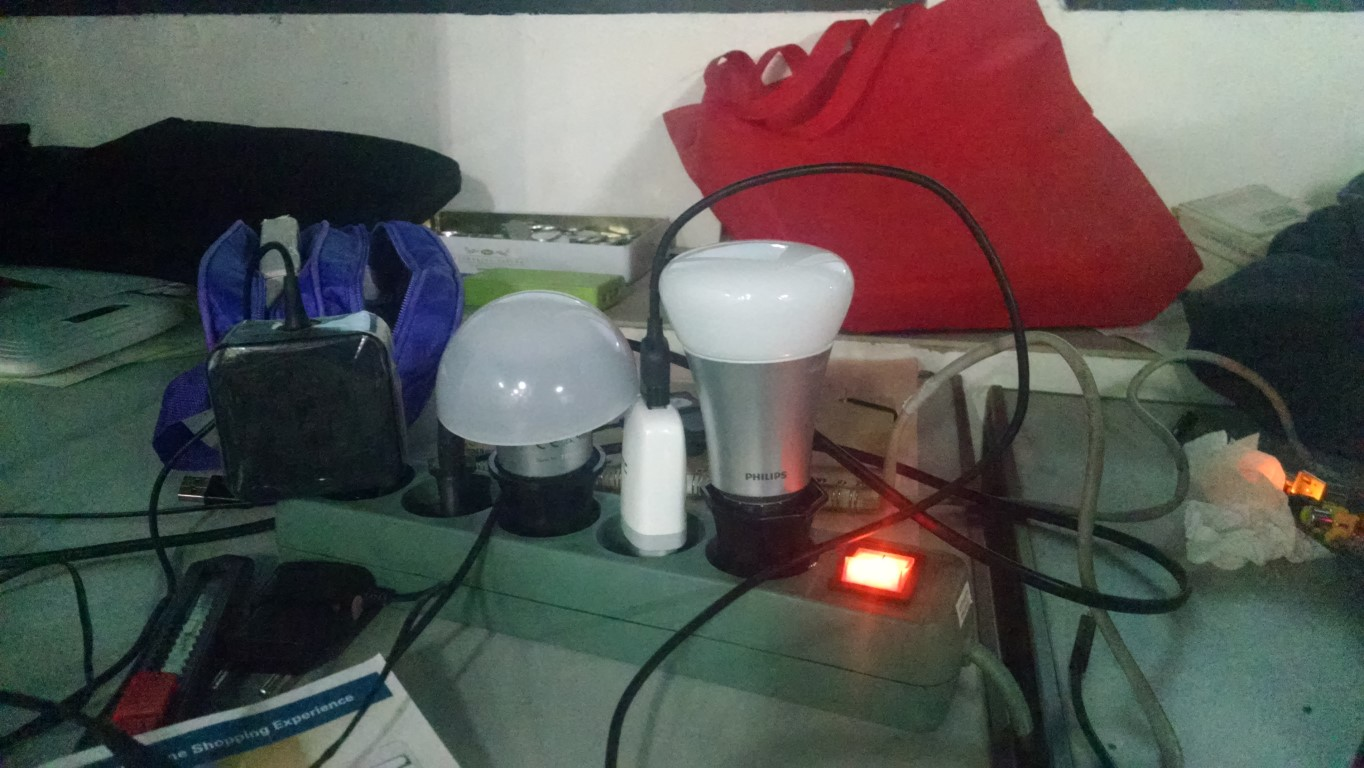
\includegraphics[width=.65\textwidth]{pics/uji9.jpg}\\
			\hline
			\textbf{Ekspektasi} & Kedua lampu mati \\
			\hline
		\end{tabular}
	\end{table}
	\item Kasus Uji 11: Mengubah tingkat kecerahan lampu dalam suatu \textit{group} melalui halaman web pada perangkat \textit{gateway}
	\begin{table}
		\centering
		\caption{Hasil pengujian kasus uji 11}
		\label{tab:kasusUji11}
		\begin{tabular}{| l | p{11cm} |}
			\hline
			\textbf{Perintah} & \textit{Slider} tingkat kecerahan pada bagian \textit{groups} digeser ke nilai yang lebih tinggi\\
			\hline
			\textbf{Prekondisi} & Perangkat \textit{gateway} sudah berjalan, lampu sudah terhubung dengan perangkat \textit{gateway}, \textit{group} sudah dibuat, dan lampu dalam keadaan menyala \\
			\hline
			\textbf{Hasil} & Kedua lampu menjadi lebih terang 
			
			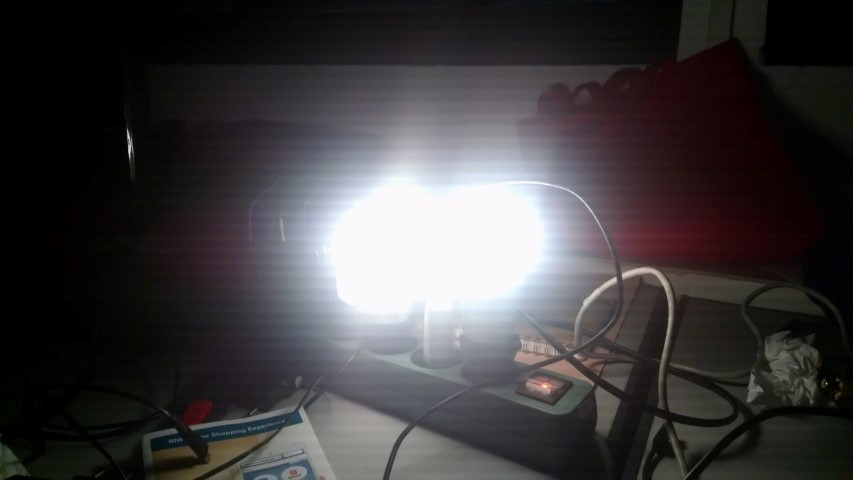
\includegraphics[width=.65\textwidth]{pics/uji10.jpg}\\
			\hline
			\textbf{Ekspektasi} & Kedua lampu menjadi lebih terang \\
			\hline
		\end{tabular}
	\end{table}
	\item Kasus Uji 12: Mengubah warna lampu dalam suatu \textit{group} melalui halaman web pada perangkat \textit{gateway}
	\begin{table}
		\centering
		\caption{Hasil pengujian kasus uji 12}
		\label{tab:kasusUji12}
		\begin{tabular}{| l | p{11cm} |}
			\hline
			\textbf{Perintah} & Mengubah warna pada \textit{color picker} menjadi berwarna hijau\\
			\hline
			\textbf{Prekondisi} & Perangkat \textit{gateway} sudah berjalan, lampu sudah terhubung dengan perangkat \textit{gateway}, \textit{group} sudah dibuat, dan lampu dalam keadaan menyala \\
			\hline
			\textbf{Hasil} & Kedua lampu menjadi berwarna hijau 
			
			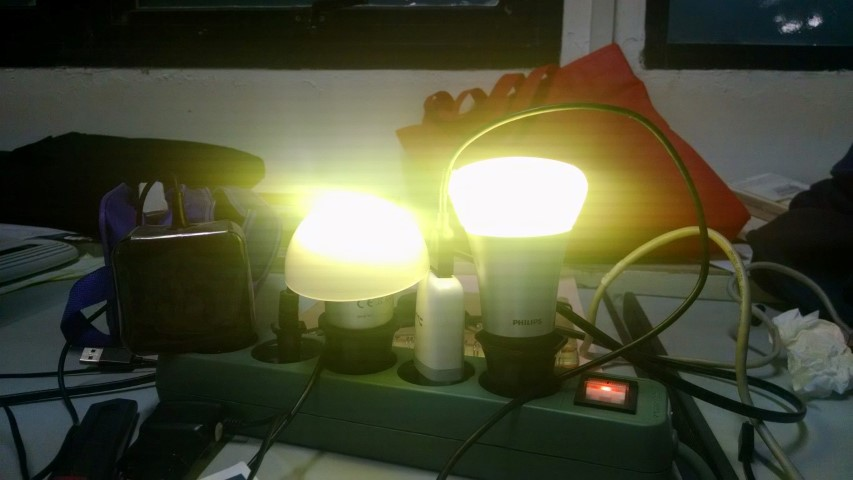
\includegraphics[width=.65\textwidth]{pics/uji11.jpg}\\
			\hline
			\textbf{Ekspektasi} & Kedua lampu menjadi berwarna hijau \\
			\hline
		\end{tabular}
	\end{table}
	\item Kasus Uji 13: Mengubah tingkat kejenuhan lampu dalam suatu \textit{group} melalui halaman web pada perangkat \textit{gateway}
	\begin{table}
		\centering
		\caption{Hasil pengujian kasus uji 13}
		\label{tab:kasusUji13}
		\begin{tabular}{| l | p{11cm} |}
			\hline
			\textbf{Perintah} & Mengubah tingkat kejenuhan warna menggunakan \textit{color picker} pada bagian \textit{groups}\\
			\hline
			\textbf{Prekondisi} & Perangkat \textit{gateway} sudah berjalan, lampu sudah terhubung dengan perangkat \textit{gateway}, \textit{group} sudah dibuat, dan lampu dalam keadaan menyala \\
			\hline
			\textbf{Hasil} & Kedua lampu menjadi berwarna berwarna lebih muda 
			
			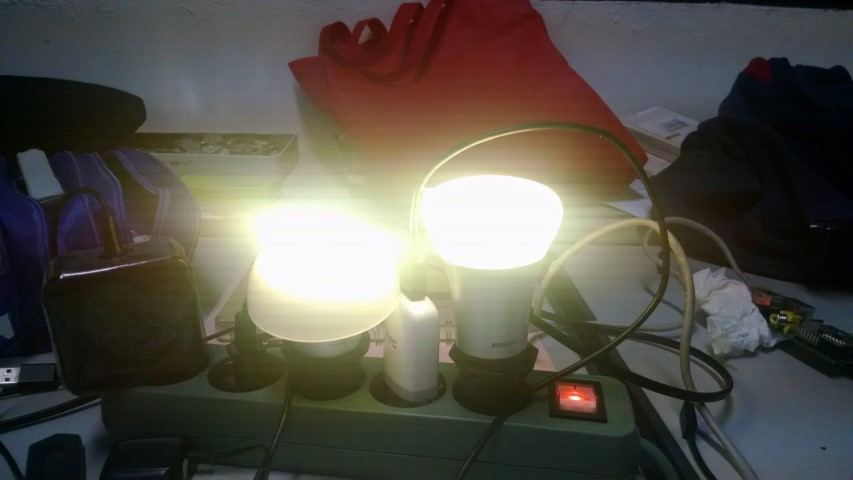
\includegraphics[width=.65\textwidth]{pics/uji12.jpg}\\
			\hline
			\textbf{Ekspektasi} & Kedua lampu menjadi berwarna berwarna lebih muda \\
			\hline
		\end{tabular}
	\end{table}
	\item Kasus Uji 14: Mendaftarkan lampu ke \plat~melalui halaman web pada perangkat \textit{gateway}.
	\begin{table}
		\centering
		\caption{Hasil pengujian kasus uji 14}
		\label{tab:kasusUji14}
		\begin{tabular}{| l | p{11cm} |}
			\hline
			\textbf{Perintah} & Menekan tombol 'Daftarkan Light2', memilih hak akses untuk setiap atribut, dan menekan tombol 'Daftar' \\
			\hline
			\textbf{Prekondisi} & Perangkat \textit{gateway} sudah terhubung ke \textit{access point} dengan koneksi internet, lampu sudah terhubung dengan perangkat \textit{gateway}\\
			\hline
			\textbf{Hasil} & Lampu beserta atribut yang dipilih terdaftar dan mendapat id \code{557d23cb0fcf33af4e209d93}\\
			\hline
			\textbf{Ekspektasi} & Lampu beserta atribut yang dipilih terdaftar dan mendapat sebuah id \\
			\hline
		\end{tabular}
	\end{table}
	\item Kasus Uji 15: Mendaftarkan \textit{group} ke \plat~melalui halaman web pada perangkat \textit{gateway}
	\begin{table}
		\centering
		\caption{Hasil pengujian kasus uji 15}
		\label{tab:kasusUji15}
		\begin{tabular}{| l | p{11cm} |}
			\hline
			\textbf{Perintah} & Menekan tombol 'Daftarkan Lab Nok', memilih hak akses untuk setiap atribut, dan menekan tombol 'Daftar' \\
			\hline
			\textbf{Prekondisi} & Perangkat \textit{gateway} sudah terhubung ke \textit{access point} dengan koneksi internet, \textit{group} sudah dibuat\\
			\hline
			\textbf{Hasil} & \textit{Group} beserta atribut yang dipilih terdaftar dan mendapat id \code{557d10c80fcf33af4e209d8e}\\
			\hline
			\textbf{Ekspektasi} & \textit{Group} beserta atribut yang dipilih terdaftar dan mendapat sebuah id \\
			\hline
		\end{tabular}
	\end{table}
	\item Kasus Uji 16: Mengirimkan informasi mengenai atribut yang didaftarkan secara berkala ke \textit{pub-sub system}
	\begin{table}
		\centering
		\caption{Hasil pengujian kasus uji 16}
		\label{tab:kasusUji16}
		\begin{tabular}{| l | p{11cm} |}
			\hline
			\textbf{Perintah} & \code{mosquitto\_sub -h 128.199.236.53 -t sot/g/557903af5ad821942ef0af51/+/+/+/acc} \\
			\hline
			\textbf{Prekondisi} & Perangkat \textit{gateway} sudah terhubung ke \textit{access point} dengan koneksi internet, lampu sudah terhubung ke perangkat \textit{gateway}\\
			\hline
			\textbf{Hasil} & Mendapatkan informasi mengenai atribut yang didaftarkan setiap sepuluh detik
			
			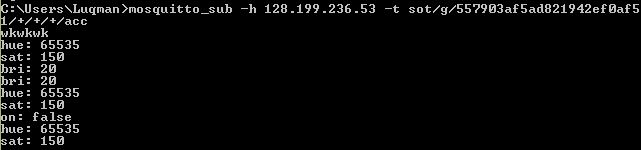
\includegraphics[width=.65\textwidth]{pics/uji15.jpg}\\
			\hline
			\textbf{Ekspektasi} & Mendapatkan informasi mengenai atribut yang didaftarkan setiap sepuluh detik \\
			\hline
		\end{tabular}
	\end{table}
	\item Kasus Uji 17: Menyalakan lampu melalui pesan yang dikirimkan dari \textit{pub-sub system}.
	\begin{table}
		\centering
		\caption{Hasil pengujian kasus uji 17}
		\label{tab:kasusUji17}
		\begin{tabular}{| l | p{11cm} |}
			\hline
			\textbf{Topik} & \code{sot/g/557903af5ad821942ef0af51/ledlight /557b693c1463cee933d9df01/on/ctl}\\
			\hline
			\textbf{Prekondisi} & Lampu sudah didaftarkan dengan atribut terkait diberikan hak kontrol, lampu dalam keadaan mati\\
			\hline
			\textbf{Isi pesan} & \code{true}\\
			\hline
			\textbf{Hasil} & Lampu menyala 
			
			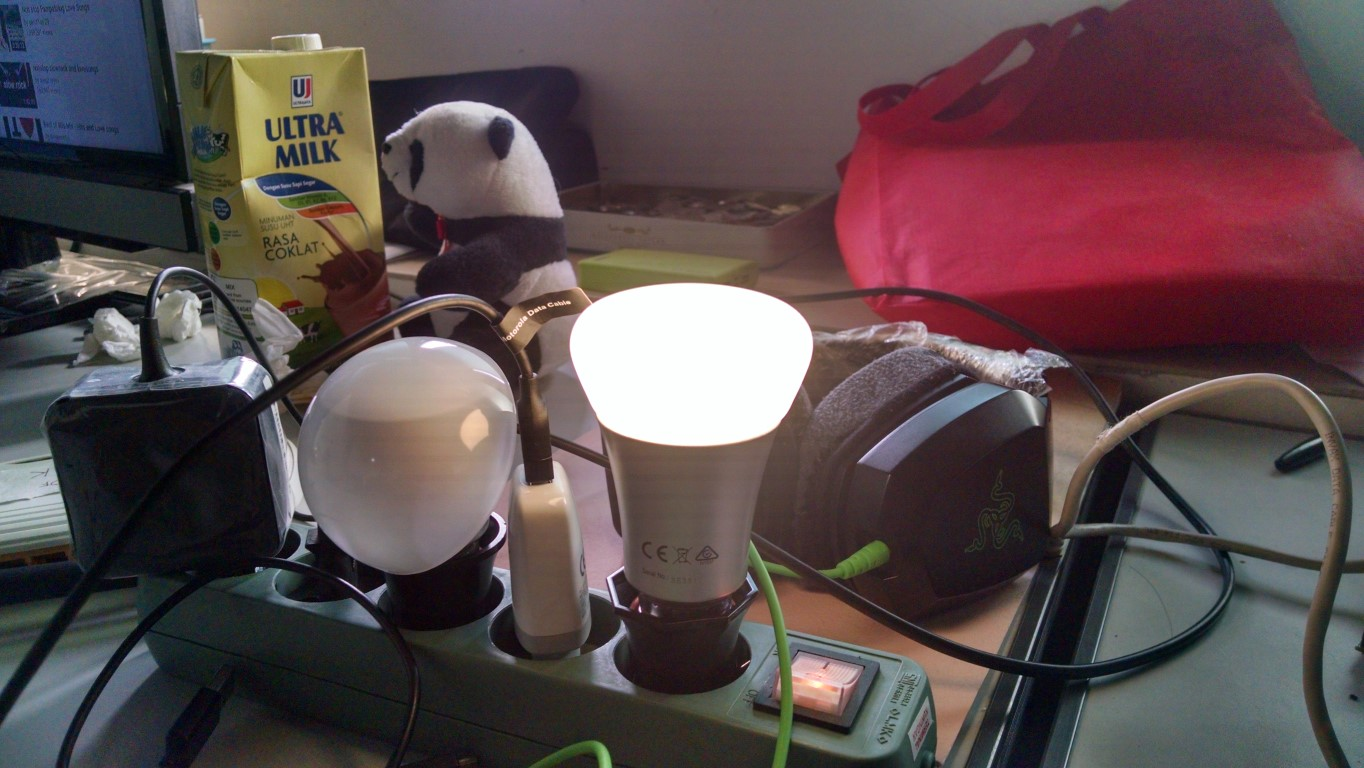
\includegraphics[width=.65\textwidth]{pics/uji16.jpg}\\
			\hline
			\textbf{Ekspektasi} & Lampu menyala \\
			\hline
		\end{tabular}
	\end{table}
	\item Kasus Uji 18: Mematikan lampu melalui pesan yang dikirimkan dari \textit{pub-sub system}.
	\begin{table}
		\centering
		\caption{Hasil pengujian kasus uji 18}
		\label{tab:kasusUji18}
		\begin{tabular}{| l | p{11cm} |}
			\hline
			\textbf{Topik} & \code{sot/g/557903af5ad821942ef0af51/ledlight /557b693c1463cee933d9df01/on/ctl}\\
			\hline
			\textbf{Prekondisi} & Lampu sudah didaftarkan dengan atribut terkait diberikan hak kontrol, lampu dalam keadaan menyala\\
			\hline
			\textbf{Isi pesan} & \code{false}\\
			\hline
			\textbf{Hasil} & Lampu mati 
			
			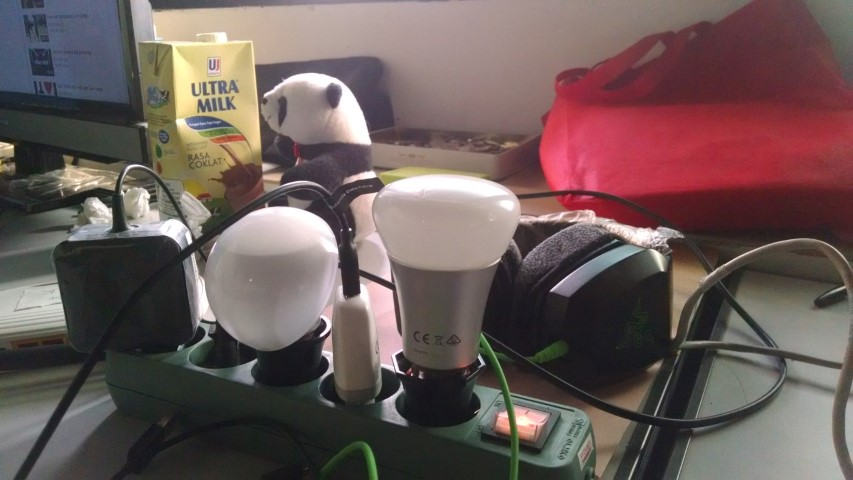
\includegraphics[width=.65\textwidth]{pics/uji17.jpg}\\
			\hline
			\textbf{Ekspektasi} & Lampu mati \\
			\hline
		\end{tabular}
	\end{table}
	\item Kasus Uji 19: Mengubah tingkat kecerahan lampu melalui pesan yang dikirimkan dari \textit{pub-sub system}.
	\begin{table}
		\centering
		\caption{Hasil pengujian kasus uji 19}
		\label{tab:kasusUji19}
		\begin{tabular}{| l | p{11cm} |}
			\hline
			\textbf{Topik} & \code{sot/g/557903af5ad821942ef0af51/ledlight /557b693c1463cee933d9df01/bri/ctl}\\
			\hline
			\textbf{Prekondisi} & Lampu sudah didaftarkan dengan atribut terkait diberikan hak kontrol, lampu dalam keadaan menyala\\
			\hline
			\textbf{Isi pesan} & \code{200}\\
			\hline
			\textbf{Hasil} & Lampu menjadi lebih terang 
			
			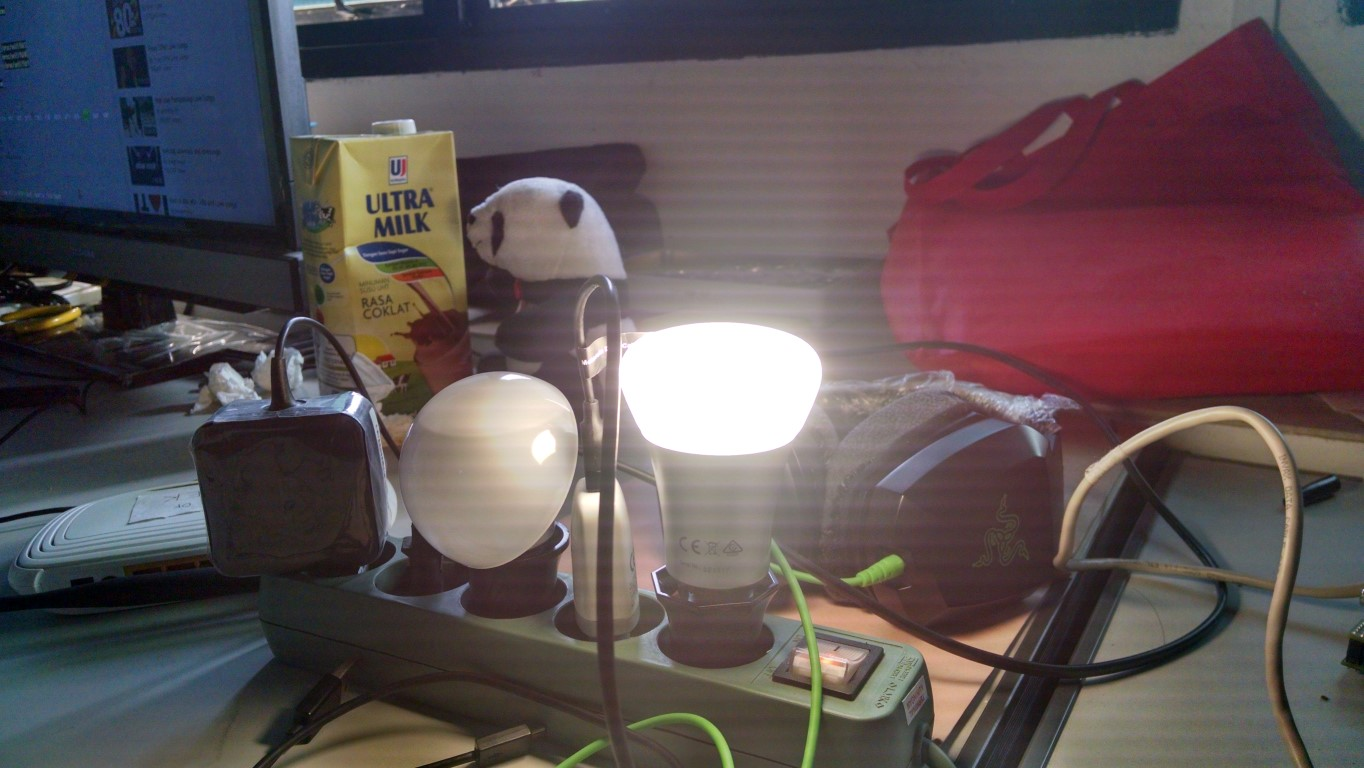
\includegraphics[width=.65\textwidth]{pics/uji18.jpg}\\
			\hline
			\textbf{Ekspektasi} & Lampu menjadi lebih terang  \\
			\hline
		\end{tabular}
	\end{table}
	\item Kasus Uji 20: Mengubah warna lampu melalui pesan yang dikirimkan dari \textit{pub-sub system}.
	\begin{table}
		\centering
		\caption{Hasil pengujian kasus uji 20}
		\label{tab:kasusUji20}
		\begin{tabular}{| l | p{11cm} |}
			\hline
			\textbf{Topik} & \code{sot/g/557903af5ad821942ef0af51/ledlight /557b693c1463cee933d9df01/hue/ctl}\\
			\hline
			\textbf{Prekondisi} & Lampu sudah didaftarkan dengan atribut terkait diberikan hak kontrol, lampu dalam keadaan menyala\\
			\hline
			\textbf{Isi pesan} & \code{45000}\\
			\hline
			\textbf{Hasil} & Lampu menjadi berwarna biru
			
			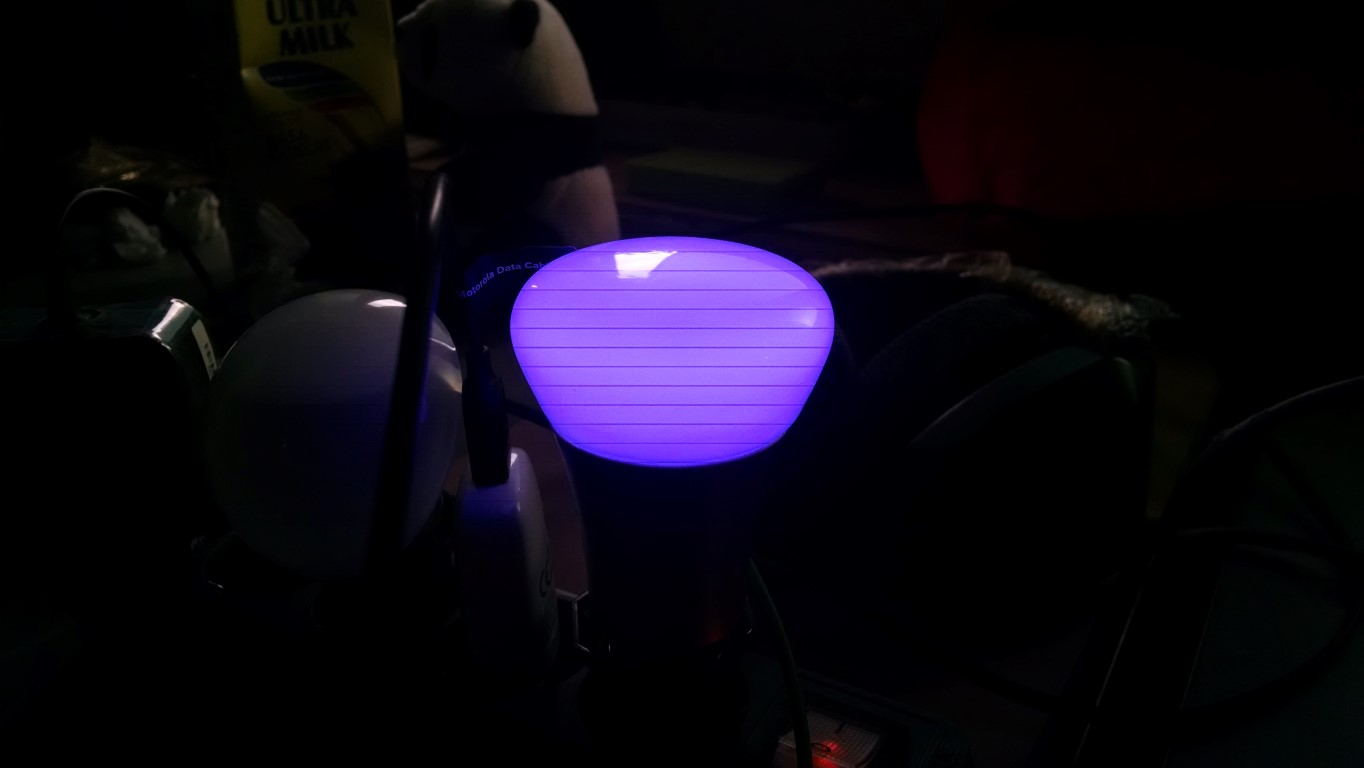
\includegraphics[width=.65\textwidth]{pics/uji19.jpg}\\
			\hline
			\textbf{Ekspektasi} & Lampu menjadi berwarna biru  \\
			\hline
		\end{tabular}
	\end{table}
	\item Kasus Uji 21: Mengubah tingkat kejenuhan lampu melalui pesan yang dikirimkan dari \textit{pub-sub system}.
	\begin{table}
		\centering
		\caption{Hasil pengujian kasus uji 21}
		\label{tab:kasusUji21}
		\begin{tabular}{| l | p{11cm} |}
			\hline
			\textbf{Topik} & \code{sot/g/557903af5ad821942ef0af51/ledlight /557b693c1463cee933d9df01/sat/ctl}\\
			\hline
			\textbf{Prekondisi} & Lampu sudah didaftarkan dengan atribut terkait diberikan hak kontrol, lampu dalam keadaan menyala\\
			\hline
			\textbf{Isi pesan} & \code{150}\\
			\hline
			\textbf{Hasil} & Lampu menjadi berwarna lebih muda
			
			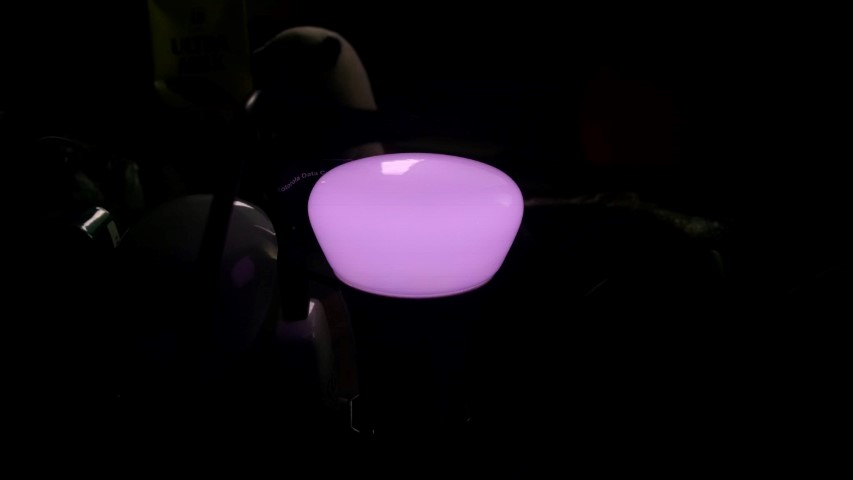
\includegraphics[width=.65\textwidth]{pics/uji20.jpg}\\
			\hline
			\textbf{Ekspektasi} & Lampu menjadi berwarna lebih muda  \\
			\hline
		\end{tabular}
	\end{table}
	\item Kasus Uji 22: Menyalakan lampu dalam suatu \textit{group} melalui pesan yang dikirimkan dari \textit{pub-sub system}.
	\begin{table}
		\centering
		\caption{Hasil pengujian kasus uji 22}
		\label{tab:kasusUji22}
		\begin{tabular}{| l | p{11cm} |}
			\hline
			\textbf{Topik} & \code{sot/g/557903af5ad821942ef0af51/ledlight /557d10c80fcf33af4e209d8e/on/ctl}\\
			\hline
			\textbf{Prekondisi} & \textit{Group} sudah didaftarkan dengan atribut terkait diberikan hak kontrol, lampu anggota \textit{group} dalam keadaan mati\\
			\hline
			\textbf{Isi pesan} & \code{true}\\
			\hline
			\textbf{Hasil} & Kedua lampu menyala 
			
			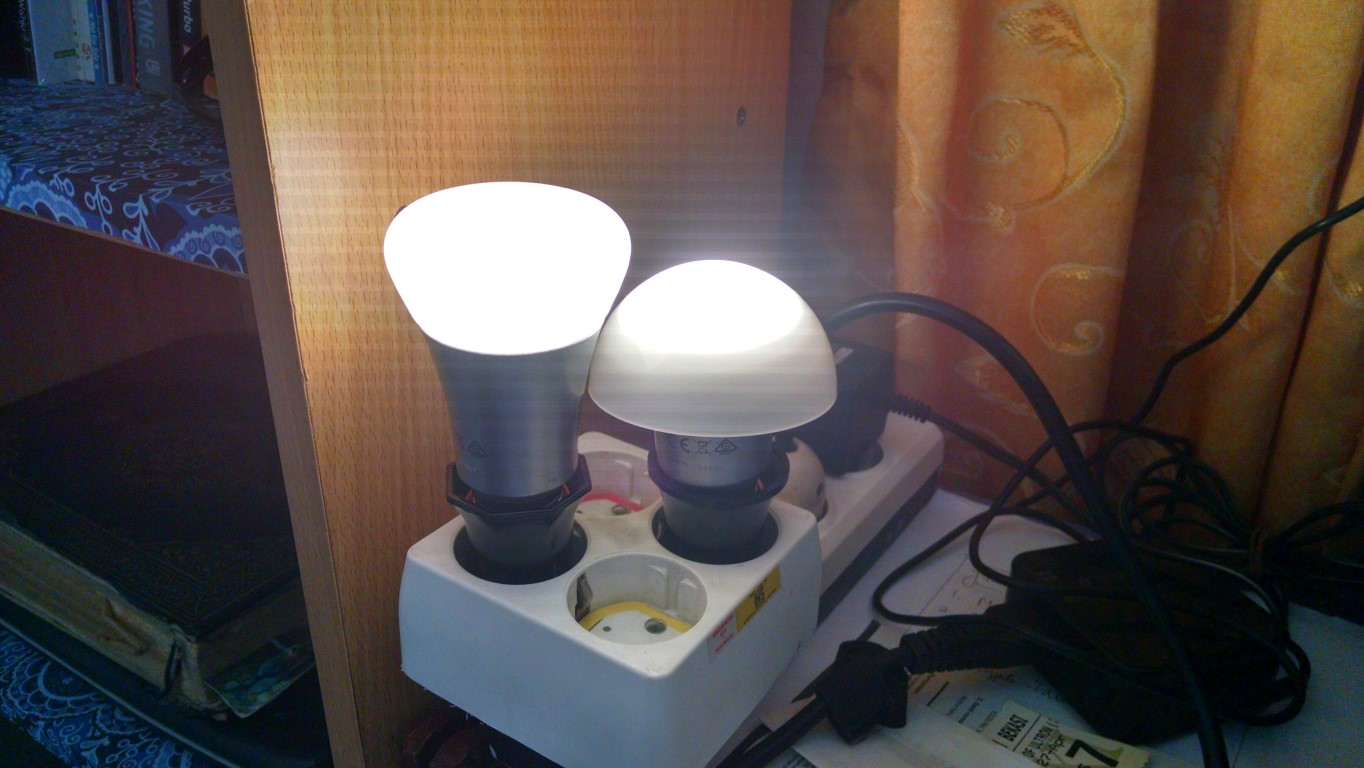
\includegraphics[width=.65\textwidth]{pics/uji21.jpg}\\
			\hline
			\textbf{Ekspektasi} & Kedua lampu menyala  \\
			\hline
		\end{tabular}
	\end{table}
	\item Kasus Uji 23: Mematikan lampu dalam suatu \textit{group} melalui pesan yang dikirimkan dari \textit{pub-sub system}.
	\begin{table}
		\centering
		\caption{Hasil pengujian kasus uji 23}
		\label{tab:kasusUji23}
		\begin{tabular}{| l | p{11cm} |}
			\hline
			\textbf{Topik} & \code{sot/g/557903af5ad821942ef0af51/ledlight /557d10c80fcf33af4e209d8e/on/ctl}\\
			\hline
			\textbf{Prekondisi} & \textit{Group} sudah didaftarkan dengan atribut terkait diberikan hak kontrol, lampu anggota \textit{group} dalam keadaan menyala\\
			\hline
			\textbf{Isi pesan} & \code{false}\\
			\hline
			\textbf{Hasil} & Kedua lampu mati 
			
			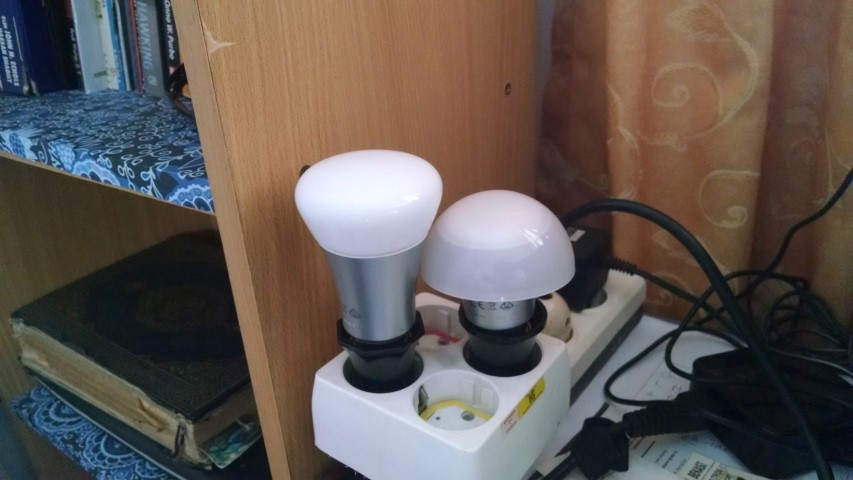
\includegraphics[width=.65\textwidth]{pics/uji22.jpg}\\
			\hline
			\textbf{Ekspektasi} & Kedua lampu mati  \\
			\hline
		\end{tabular}
	\end{table}
	\item Kasus Uji 24: Mengubah tingkat kecerahan lampu dalam suatu \textit{group} melalui pesan yang dikirimkan dari \textit{pub-sub system}.
	\begin{table}
		\centering
		\caption{Hasil pengujian kasus uji 24}
		\label{tab:kasusUji24}
		\begin{tabular}{| l | p{11cm} |}
			\hline
			\textbf{Topik} & \code{sot/g/557903af5ad821942ef0af51/ledlight /557d10c80fcf33af4e209d8e/bri/ctl}\\
			\hline
			\textbf{Prekondisi} & \textit{Group} sudah didaftarkan dengan atribut terkait diberikan hak kontrol, lampu anggota \textit{group} dalam keadaan menyala\\
			\hline
			\textbf{Isi pesan} & \code{200}\\
			\hline
			\textbf{Hasil} & Kedua lampu menjadi lebih terang
			
			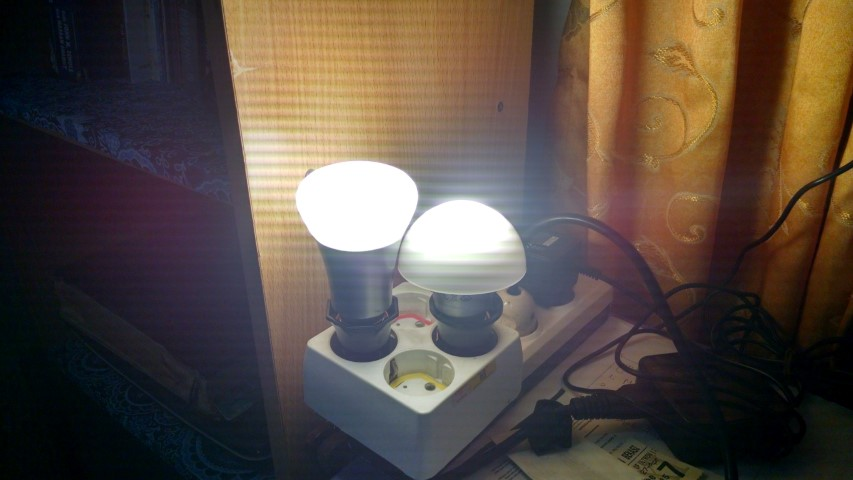
\includegraphics[width=.65\textwidth]{pics/uji23.jpg}\\
			\hline
			\textbf{Ekspektasi} & Kedua lampu menjadi lebih terang  \\
			\hline
		\end{tabular}
	\end{table}
	\item Kasus Uji 25: Mengubah warna lampu dalam suatu \textit{group} melalui pesan yang dikirimkan dari \textit{pub-sub system}.
	\begin{table}
		\centering
		\caption{Hasil pengujian kasus uji 25}
		\label{tab:kasusUji25}
		\begin{tabular}{| l | p{11cm} |}
			\hline
			\textbf{Topik} & \code{sot/g/557903af5ad821942ef0af51/ledlight /557d10c80fcf33af4e209d8e/hue/ctl}\\
			\hline
			\textbf{Prekondisi} & \textit{Group} sudah didaftarkan dengan atribut terkait diberikan hak kontrol, lampu anggota \textit{group} dalam keadaan menyala\\
			\hline
			\textbf{Isi pesan} & \code{65535}\\
			\hline
			\textbf{Hasil} & Kedua lampu menjadi berwarna merah
			
			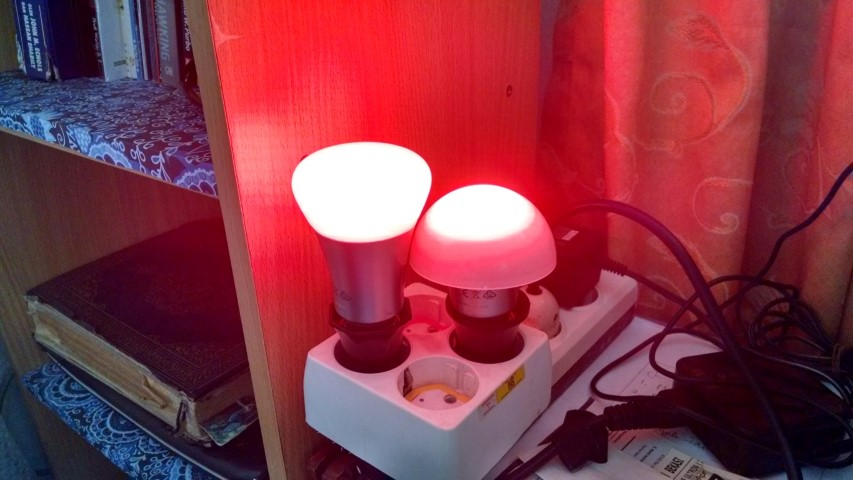
\includegraphics[width=.65\textwidth]{pics/uji24.jpg}\\
			\hline
			\textbf{Ekspektasi} & Kedua lampu menjadi berwarna merah  \\
			\hline
		\end{tabular}
	\end{table}
	\item Kasus Uji 26: Mengubah tingkat kejenuhan lampu dalam suatu \textit{group} melalui pesan yang dikirimkan dari \textit{pub-sub system}.
	\begin{table}
		\centering
		\caption{Hasil pengujian kasus uji 26}
		\label{tab:kasusUji26}
		\begin{tabular}{| l | p{11cm} |}
			\hline
			\textbf{Topik} & \code{sot/g/557903af5ad821942ef0af51/ledlight /557d10c80fcf33af4e209d8e/sat/ctl}\\
			\hline
			\textbf{Prekondisi} & \textit{Group} sudah didaftarkan dengan atribut terkait diberikan hak kontrol, lampu anggota \textit{group} dalam keadaan menyala\\
			\hline
			\textbf{Isi pesan} & \code{150}\\
			\hline
			\textbf{Hasil} & Kedua lampu menjadi berwarna lebih muda
			
			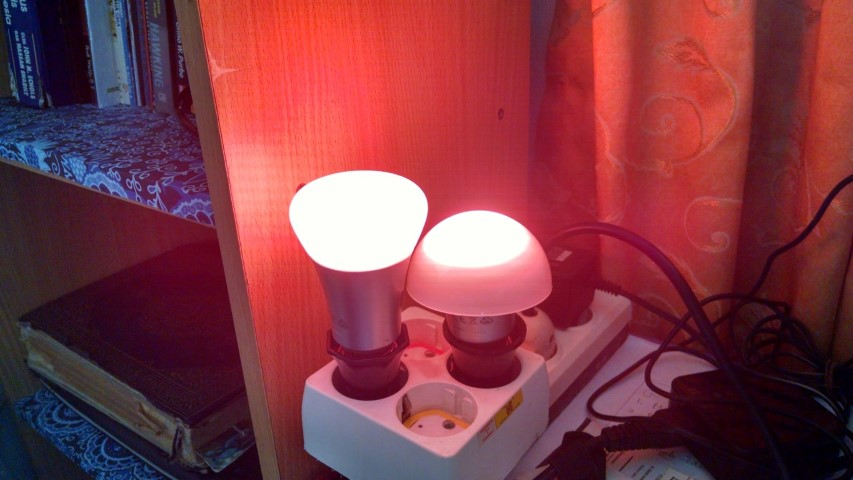
\includegraphics[width=.65\textwidth]{pics/uji25.jpg}\\
			\hline
			\textbf{Ekspektasi} & Kedua lampu menjadi berwarna lebih muda  \\
			\hline
		\end{tabular}
	\end{table}
\end{enumerate}